

\section{Application to compact finite differences}

\begin{frame}
\frametitle{Application to compact finite difference schemes}
\begin{itemize}
\item Compact finite difference evaluation involves two steps:
    \begin{enumerate}
        \item Evaluation of the right hand sides
        \begin{itemize}
            \item easily performed on the GPU
        \end{itemize}
        \item Solving the tridiagonal systems for all the grid lines
    \end{enumerate}
\item Typical DNS problems too large to fit on a single GPU
\item Need a strategy for multiple GPUs
\end{itemize}
\end{frame}

\begin{frame}
\frametitle{Parallelization strategy: single GPU}
\begin{columns}
\begin{column}{0.5\textwidth}
\begin{itemize}
    \item Map grid lines to blocks
    \item Solve multiple blocks simaltaneously
    \item For other coordinate directions,
        transpose the data (physically or logically)
\end{itemize}
\end{column}
\begin{column}{0.5\textwidth}
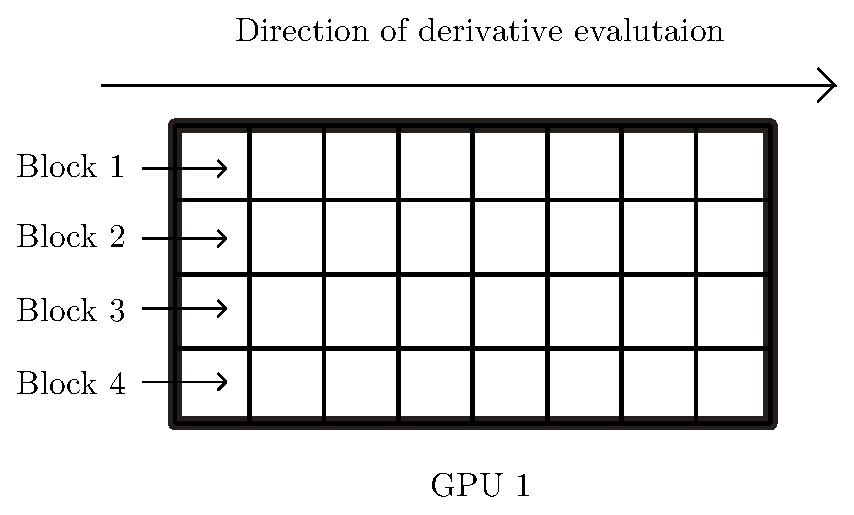
\includegraphics[width=150px]{img/compact-single-gpu.eps}
\end{column}
\end{columns}
\end{frame}

\begin{frame}
\frametitle{Parallelization strategy: multiple GPUs on a single node}
\begin{columns}
\begin{column}{0.5\textwidth}
\begin{itemize}
\item Method used by Sakharnykh et al.
\item Decompose domain into \emph{subdomains};
    each GPU assigned a subdomain
\item Single subdomain used along derivative direction
\item No coordination between GPUs required
\item For other coordinate directions,
    transpose the data (physically or logically)
\end{itemize}
\end{column}
\begin{column}{0.5\textwidth}
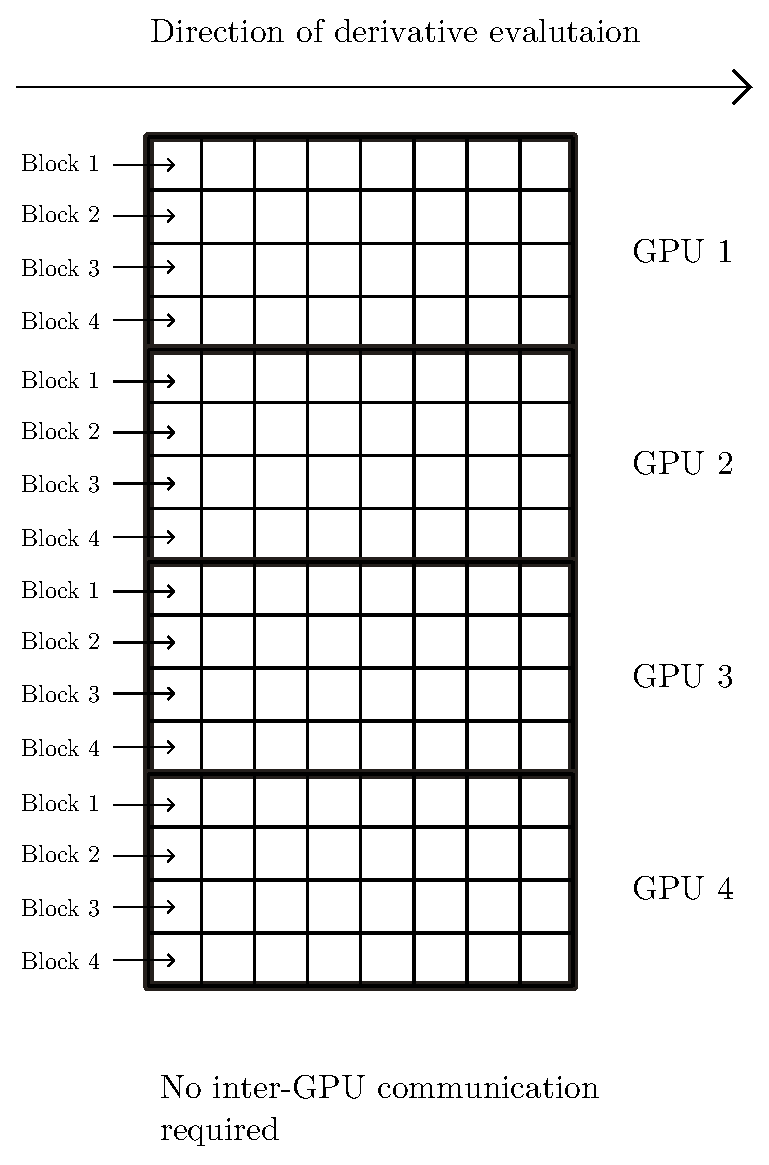
\includegraphics[width=100px]{img/compact-shared-gpu.eps}
\end{column}
\end{columns}
\end{frame}

\begin{frame}
\frametitle{Parallelization strategy: multiple GPUs on distinct nodes}
\begin{columns}
\begin{column}{0.5\textwidth}
\begin{itemize}
\item Single subdomain used along derivative direction
\item No coordination between GPUs required
\item \textbf{Physical} global transpose required
\item Subdomains can become impractically slender
\end{itemize}
\end{column}
\begin{column}{0.5\textwidth}
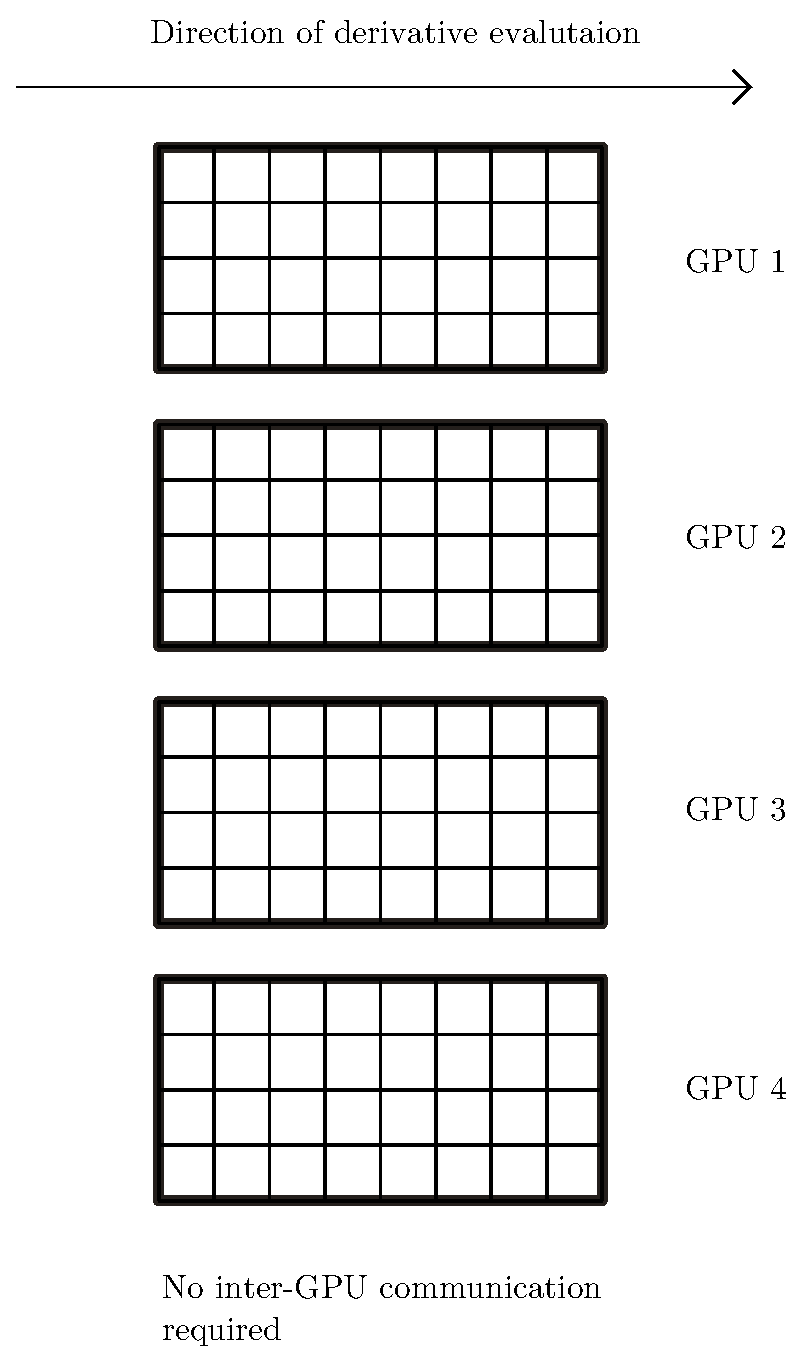
\includegraphics[width=100px]{img/compact-distributed-restricted.eps}
\end{column}
\end{columns}
\end{frame}

\begin{frame}
\frametitle{Parallelization strategy: multiple GPUs on distinct nodes}
\centering
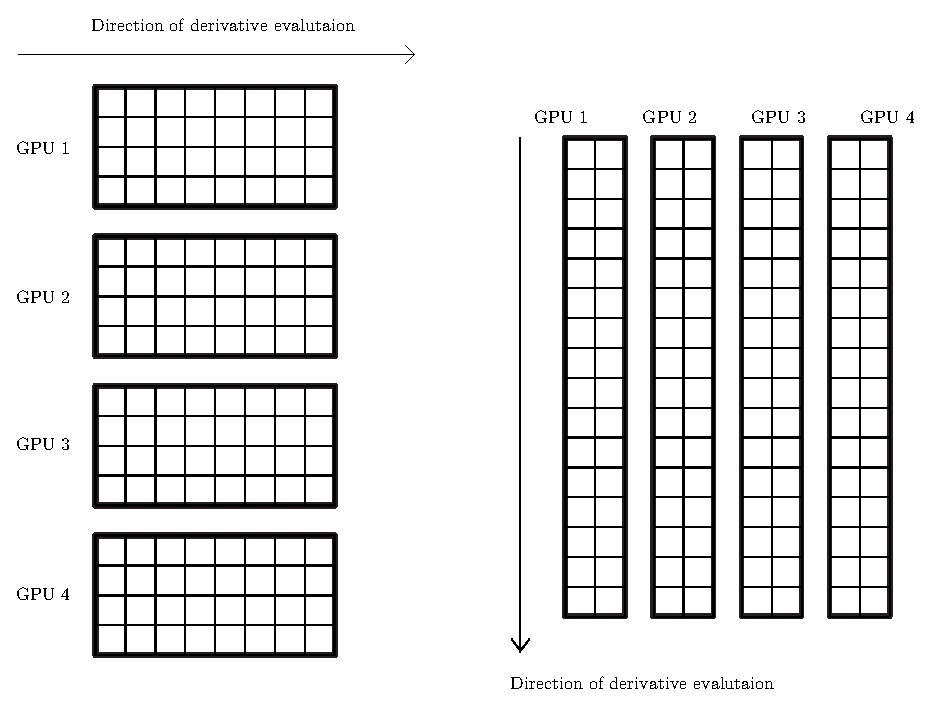
\includegraphics[width=200px]{img/compact-restricted-transpose.eps}
\end{frame}

\begin{frame}
\frametitle{Parallelization strategy: multiple GPUs on distinct nodes}
\begin{columns}
\begin{column}{0.5\textwidth}
\begin{itemize}
\item Need a distributed tridiagonal solver
\item Can ease communication costs
\item Remove restrictions on domain sizes
\item Greatly increases overall complexity
\item Especially difficult for GPUs
\end{itemize}
\end{column}
\begin{column}{0.5\textwidth}
\centering
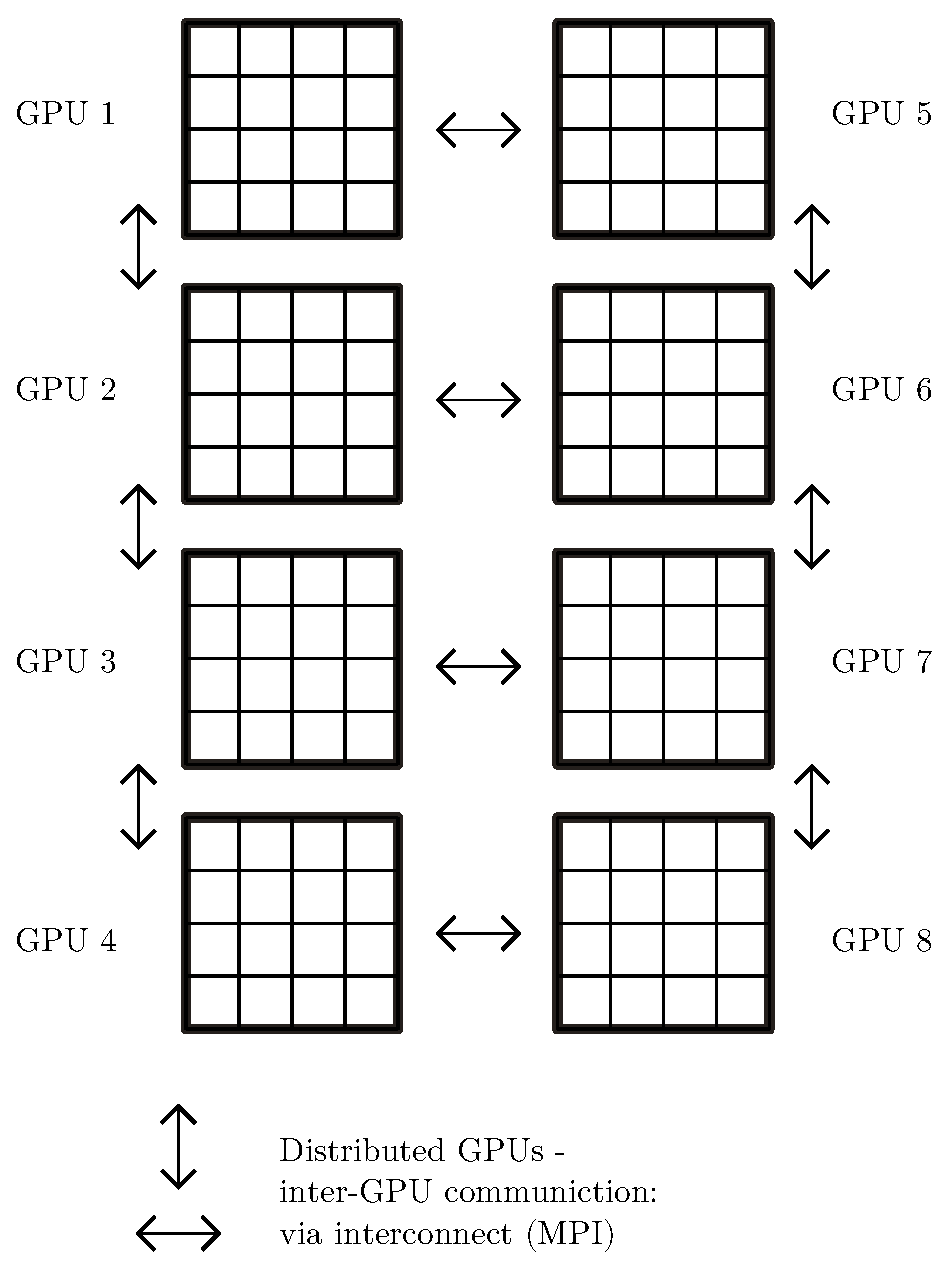
\includegraphics[width=100px]{img/compact-distributed-all.eps}
\end{column}
\end{columns}
\end{frame}

\begin{frame}
\frametitle{Distributed tridiagonal solver}

Solving a tridiagonal system of size
$mP$, split among $P$ processes:

\footnotesize
\begin{columns}
\begin{column}{0.5\textwidth}
\begin{enumerate}
\item Each process solves the local systems:
    \begin{align*}
        A^px_r^{p} &= r_p \\
        A^pu^p &= \{-a_1^p, 0, 0, 0, \hdots\} \\
        A^pl^p &= \{0, 0, 0 \hdots, -c_m^p\}
    \end{align*}
\item Construct and assemble a ``reduced'' system
    of the form:
    \scalebox{0.6}{
        \vbox{
    \begin{align*}
     \begin{bmatrix}
l^1_m & -1 \\
-1    & u^2_1 & l^2_1 \\
  & u^2_m & l^2_m & -1 \\
  &       & -1    & u^3_1 & l^3_1 \\
  &       &       & u^3_m & l^3_m  & -1 \\
  &       &       &       & \ddots & \ddots & \ddots \\
  &       &       &       &        & -1     & u^P_1
\end{bmatrix}
\begin{bmatrix}
\beta^1 \\
\alpha^2 \\
\beta^2 \\
\alpha^3 \\
\beta^3 \\
\vdots \\
\alpha^P
\end{bmatrix}
=
\begin{bmatrix}
x_{r,m}^1 \\
x_{r,1}^2 \\
x_{r,m}^2 \\
x_{r,1}^3 \\
x_{r,m}^3 \\
\vdots \\
x_{r,1}^P \\
\end{bmatrix}  
        \end{align*}}}
\item Local part of solution given by:
\begin{align*}
x^p = x_r^p + \
    \alpha^p u^p + \beta^p l^p
\end{align*}
\end{enumerate}
\end{column}
\begin{column}{0.5\textwidth}
\centering
\includegraphics[width=120px]{img/dividing-tridiagonal.eps}
\end{column}
\end{columns}
\end{frame}

\begin{frame}
\begin{itemize}
\item 3 local tridiagonal systems ($m$ equations)
\item 1 ``global'' tridiagonal system ($2P-2$ equations)
\item Must be done for each grid line
\item Sufficient to consider a single line of processes
\end{itemize}
\begin{center}
\includegraphics[height=100px]{img/single-line-of-processes.eps}
\end{center}
\end{frame}

\begin{frame}
\frametitle{Right hand side evaluation}
\begin{columns}
\begin{column}{0.5\textwidth}
\begin{itemize}
\item Stencil pattern: easily performed on GPU
\item Each process communicates with its neighbours
    (halo-swapping)
\item NVIDIA GPUDirect technology for efficient
    GPU-GPU communication
\item Developed a tool to manage structured grid data
    and transparently perform halo swaps
    for multiple GPUs
\end{itemize}
\end{column}
\begin{column}{0.5\textwidth}
\includegraphics[width=150px]{img/rhs-halos.eps}
\end{column}
\end{columns}
\end{frame}

\begin{frame}
\frametitle{Solving local systems}
\begin{itemize}
\item Local tridiagonal systems solved using
    algorithm described in previous sections
\item For 2-D problems,
    $N_{rhs} = m$
    for 3-D problems
    $N_{rhs} = m^2$
\end{itemize}
\end{frame}

\begin{frame}
\frametitle{Constructing reduced system}
\begin{columns}
\begin{column}{0.5\textwidth}
\begin{itemize}
\item Involves global communication
\item Produces tridiagonal system with
    several right-hand sides
\item Systems are \emph{interleaved}
\item Solved by thread-parallel Thomas
    (pThomas) algorithm
\end{itemize}
\end{column}
\begin{column}{0.5\textwidth}
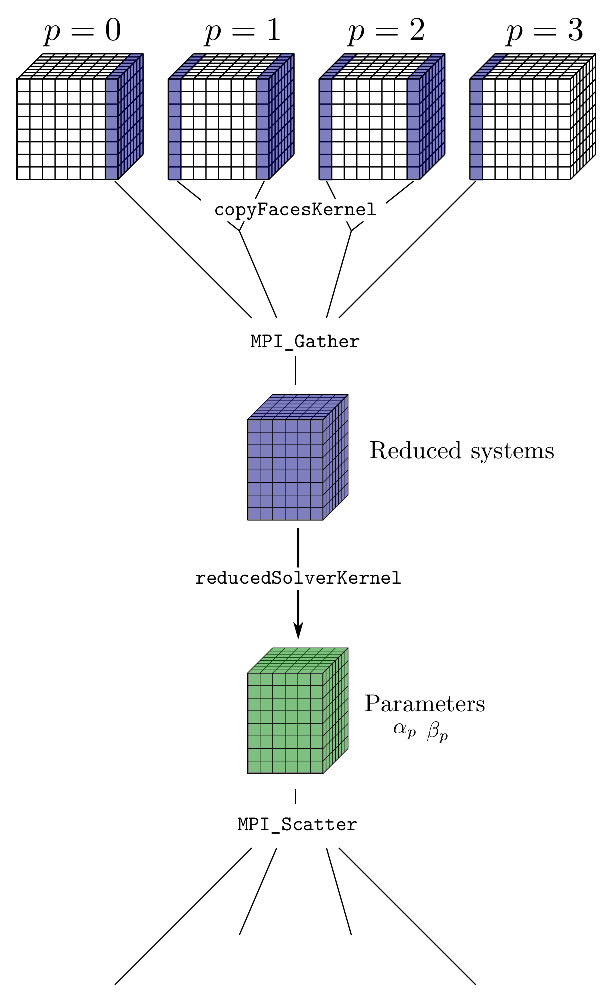
\includegraphics[width=100px]{img/constructing-reduced-system.eps}
\end{column}
\end{columns}
\end{frame}

\begin{frame}
\frametitle{Summing the solutions}
\begin{itemize}
\item Pointwise-parallel: perfect fit for GPU
\item No communication involved
\end{itemize}
\end{frame}
